\section{H69: Restatement loops copy the context window}

\textbf{The question:} In some weeks, agents restate their own earlier statements again and again. Does such a loop start when the agent's context fills with its own output? Does it end when the context is erased, or when new input arrives?

\textbf{The intuition:} Picture a spin with a self-coupling: once it points one way, it pulls itself to stay there. A fixed point is a state that the dynamics maps back onto itself. H69 proposed that a restatement loop is a fixed point of the agent's context. The agent reads its own recent text and writes it again. If the loop lives in the context window, then an erasure (the scaffold clears the context) should break it. New messages from the room should dilute the agent's own text and also help. In information terms, a restatement is copying, not transformation.

\textbf{What we measured:} We mapped 55k regime-III chat statements to their model calls and context segments (the stretch between two context resets). Nine goal periods qualified, and four had at least 30 loop episodes. The decisive observable is an odds ratio. It compares two kinds of earlier own statement at matched agent, lag and call distance. Is one still in context copied more often than one an erasure removed? Onset and exit models used agent fixed effects. For the scheduler, the control is calls between statements, not minutes, and first statements of a day are not at risk. For the external drive, a variant drops templated and echoed statements, and G51 treats operator input as the drive. For the shared model prior, agent fixed effects and a context-fill control enter every model. For common input, only cross-call restatements count, and messages posted but not yet read serve as a placebo. A synthetic check on the real call skeletons came first. It separated H69 from a recency null and from an input-starvation rival, and it showed that the threshold test had no power.

\textbf{What we found:} The claim is half right. A statement still in context is near-copied $3.38\times$ [2.56, 4.46] more often than an erased one. This holds in 4 of 4 scorable periods ($I^2=0$) and with both embedding models (bge 3.5, gte 6.1). A fake boundary in the middle of a segment gives 1.11 [0.98, 1.26]. A forced erasure, timed by the scaffold at the 41-call cap (NE41), raises loop exit $2.40\times$ [1.18, 4.88] and lowers onset to $0.54\times$ [0.34, 0.86]. The trigger is not the self-share: room messages in context do not dilute it. Novel input does not end loops (exit 1.23 [0.85, 1.78], no larger than the unread placebo). In G51, nudges read inside a loop give 0.81 [0.49, 1.34]. Scope: G38, G40, G41, G51. The claim that stands is ``restatement loops are copies held by the context window''\cred{0.85}, EU 2.34. One small conflict: the metadata quotes the fake-boundary control as 1.13 (round~1). The card's latest round, the segment-cut recheck, gives 1.11, used here.

\begin{figure}[h]
\includegraphics[width=\textwidth]{H69-restatement-loops/fig.pdf}
\caption{Restatement loops copy what is still in the context window. (a) A schematic: an agent's own statements on the call clock; an erasure removes the older ones from its context. (b) The odds that a statement copies an in-context source rather than an erased one, per goal period. The gray fake-boundary null sits near 1, and the pool is 3.38. (c) A forced erasure raises the odds that a loop ends $2.40\times$ and lowers the odds that one starts to $0.54\times$.}
\end{figure}
\begin{figure}[h]
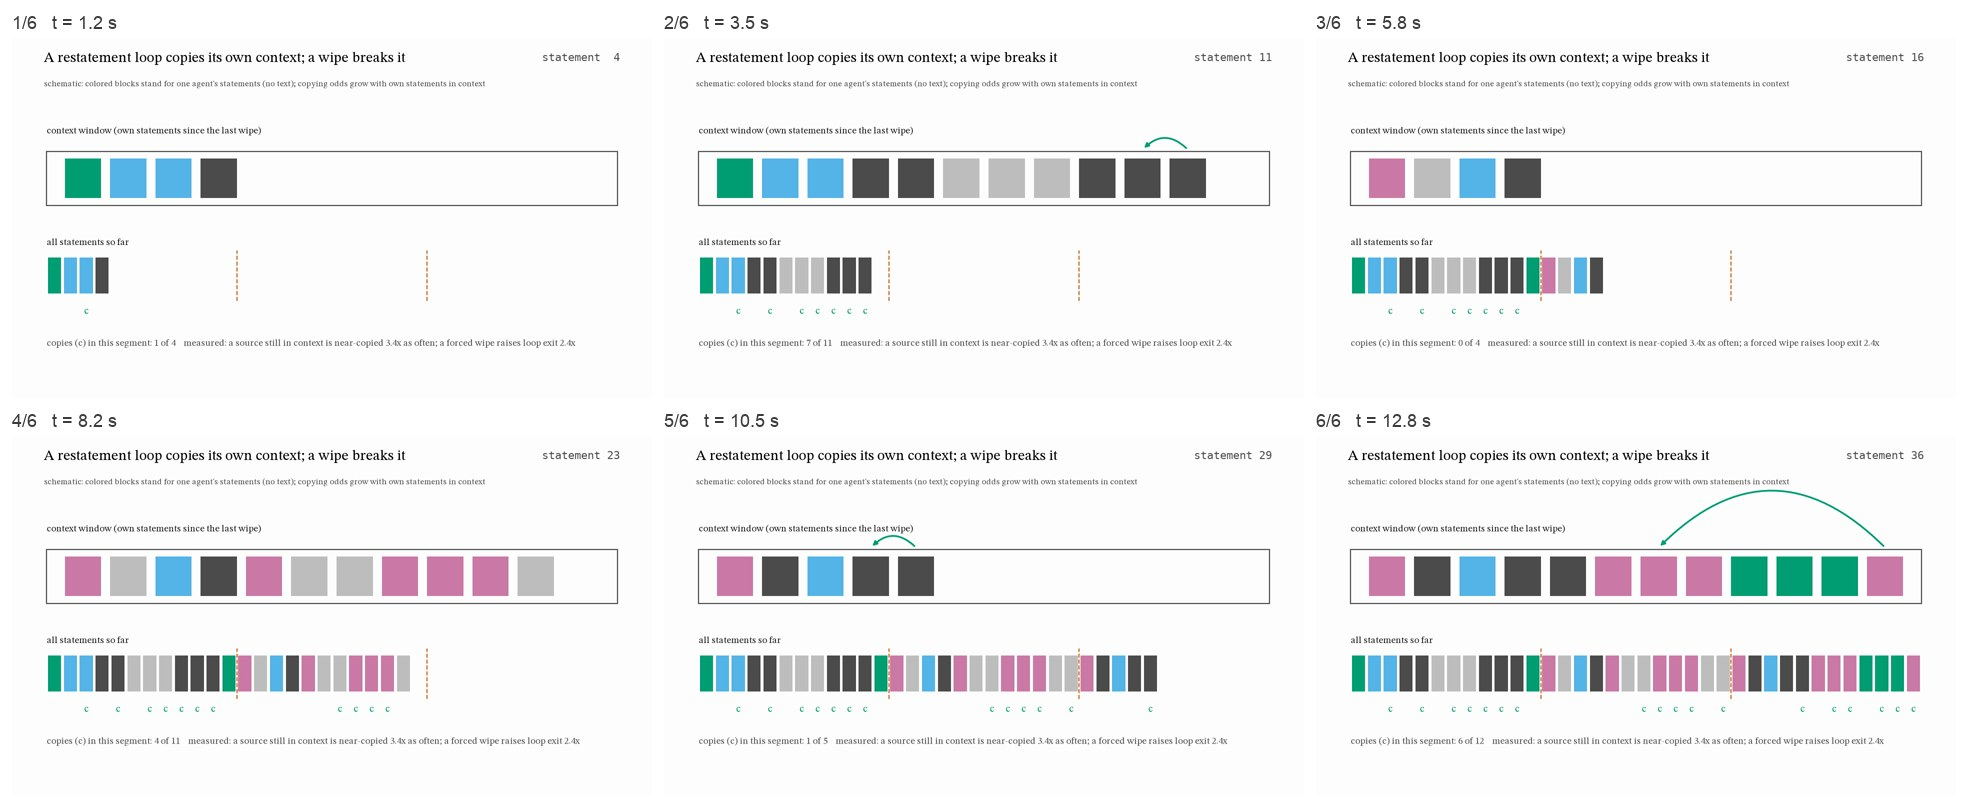
\includegraphics[width=0.9\textwidth]{storyboards/H69.jpg}
\caption{Animation storyboard: six frames of the animation, evenly spaced in time (frame number and time above each). The full animation is \texttt{writeup/animations/H69-restatement-loops.mp4}.}
\end{figure}


\noindent Animation: \texttt{writeup/animations/H69-restatement-loops.mp4}.

\textbf{What it means:} For an operator: to break a restatement loop, erase or trim the agent's context. One forced erasure more than doubles the exit odds and halves the onset odds. Do not rely on messages: nudges read inside a loop do not help (0.81). A busy room does not protect an agent either. For a scaffold builder: cap the agent's own chat kept in context, for example by dropping its oldest self-messages. Each doubling of the agent's own statements in its window raises onset odds by about $\times1.25$. The 41-call cap already acts as a loop breaker, at a cost of 4--10\% of output (H44).

\textbf{Caveats:} Only four periods have at least 30 loop episodes. The erasure exit effect varies across them ($I^2=0.74$; G51 1.36, not significant). The effect size depends on the embedding model. The self-share counts chat items, not the agent's tool output, which dominates prompt tokens. Memory and artifacts may still carry erased statements, so the enrichment is a lower bound. The threshold test (P2) had no power. Context fill also raises onset, which links to H46's style drift. The confirmation script is written and dry-run; no confirmation test on reserved goal periods has run yet.
